\documentclass[conference]{IEEEtran}

% ---- packages ----
\usepackage[utf8]{inputenc}
\usepackage[T1]{fontenc}
\usepackage{amsmath,amssymb}
\usepackage{graphicx}
\usepackage{booktabs}
\usepackage{hyperref}
\usepackage{cite}
\usepackage{algorithm}
\usepackage{algorithmic}
\usepackage{xcolor}
\usepackage{multirow}
\usepackage{enumitem}

\graphicspath{{../figures/}}

% ---- metadata ----
\title{Reinforcement Learning for Autonomous Penetration Testing:\\
       A Comparative Study of DQN and PPO with Curriculum Learning}

\author{
  \IEEEauthorblockN{Vinay Appajigowda}
  \IEEEauthorblockA{
    Student ID: x24262013\\
    National College of Ireland\\
    Dublin, Ireland\\
    \texttt{x24262013@student.ncirl.ie}
  }
}

\begin{document}

\maketitle

% ==================================================================
\begin{abstract}
Automated penetration testing is essential for proactive cyber-security,
yet manual assessments are time-consuming and inconsistent.  This paper
investigates two deep reinforcement learning (RL) algorithms---Deep
Q-Network (DQN) and Proximal Policy Optimization (PPO)---for autonomous
network penetration testing in a custom simulated environment inspired by
PenGym.  We introduce a \emph{curriculum learning} strategy where agents
are first trained on small networks (10 hosts) before being transferred
to progressively larger topologies (20, 30, and 50 hosts).  Experimental
results show that (i) PPO converges more reliably than DQN on medium-size
networks, (ii) curriculum-trained agents generalize better to unseen
large networks compared to agents trained from scratch, and (iii) both
algorithms exhibit graceful performance degradation as network complexity
increases.  Our findings contribute to the growing body of work on
RL-driven offensive security automation.
\end{abstract}

\begin{IEEEkeywords}
reinforcement learning, penetration testing, deep Q-network,
proximal policy optimization, curriculum learning, cyber-security
\end{IEEEkeywords}

% ==================================================================
\section{Introduction}
\label{sec:intro}

Penetration testing is a controlled process of exploiting
vulnerabilities in computer networks to assess their security
posture~\cite{ghanem2023jiis}.  Traditional penetration testing relies
heavily on human expertise and is both expensive and difficult to
scale~\cite{alhamed2025ijacsa}.  Reinforcement learning (RL) offers a
promising path toward automating this process by allowing agents to learn
attack strategies through interaction with simulated
environments~\cite{nguyen2025cose}.

Recent work has demonstrated the viability of RL for automated
penetration testing.  Ghanem \emph{et al.}~\cite{ghanem2023jiis}
applied hierarchical RL for efficient penetration testing of large networks, while Oh \emph{et
al.}~\cite{oh2024electronics} explored deep RL for cyber-attack simulation.  Liu \emph{et al.}~\cite{liu2024electronics} proposed hierarchical RL frameworks for automated testing, and Terranova \emph{et
al.}~\cite{terranova2024raid} addressed cyber-attack path prediction through deep RL.

Despite these advances, two challenges remain under-explored:
\begin{enumerate}[noitemsep]
  \item \textbf{Algorithm comparison:}  Systematic side-by-side
        evaluation of value-based (DQN) and policy-gradient (PPO)
        methods under identical conditions.
  \item \textbf{Scalability via curriculum learning:}  Training on
        small networks and transferring knowledge to larger, unseen
        topologies.
\end{enumerate}

This paper addresses both gaps.  Our contributions are:
\begin{itemize}[noitemsep]
  \item A custom, configurable network penetration testing environment
        supporting 10 to 50+ hosts with stochastic vulnerability
        exploitation.
  \item A rigorous comparison of DQN and PPO across multiple network
        sizes.
  \item A curriculum learning pipeline that improves generalization to
        large networks.
\end{itemize}

% ==================================================================
\section{Related Work}
\label{sec:related}

\textbf{RL for penetration testing.}
Alhamed and Rahman~\cite{alhamed2025ijacsa} apply DQN and quantile-regression DQN to automated DoS penetration testing, demonstrating effective policy learning.  AlMajali \emph{et al.}~\cite{almajali2024applsci} investigate automated vulnerability exploitation using deep reinforcement learning in simulated enterprise networks.

\textbf{Deep RL methods.}
Liu \emph{et al.}~\cite{liu2024electronics} propose an automated penetration testing framework based on hierarchical reinforcement learning, reporting faster convergence than flat approaches.  Sun \emph{et al.}~\cite{sun2025plosone} combine ontology knowledge with reinforcement learning for intelligent penetration testing in power IoT systems.  Oh \emph{et al.}~\cite{oh2024electronics} employ deep RL for cyber-attack simulation to enhance cybersecurity assessment.

\textbf{Scalability and curriculum learning.}
Moreno \emph{et al.}~\cite{moreno2025sensors} analyse autonomous penetration testing through reinforcement learning combined with recommender systems.  Terranova \emph{et al.}~\cite{terranova2024raid} leverage deep RL for cyber-attack path prediction, addressing formulation, generalisation, and evaluation.  Nguyen \emph{et al.}~\cite{nguyen2025cose} present PenGym, a realistic training environment for RL pentesting agents with support for transfer learning between network sizes.

% ==================================================================
\section{Methodology}
\label{sec:method}

\subsection{Environment Design}

We implement a custom network penetration testing environment
(Fig.~\ref{fig:summary}) inspired by PenGym~\cite{terranova2024raid}.
Each environment instance is parameterized by:
\begin{itemize}[noitemsep]
  \item $N$ hosts connected by a random adjacency graph with
        configurable connectivity;
  \item $V$ vulnerabilities distributed across hosts, each with a
        difficulty parameter $d \in [0.2, 0.95]$;
  \item optional adjacency requirements: some vulnerabilities can only
        be exploited if a neighbouring host is already compromised.
\end{itemize}

The agent starts with access to a single entry-point host and must
discover and exploit vulnerabilities to compromise the entire network.
At each step, the agent may \emph{scan} a reachable host (revealing
its vulnerabilities) or \emph{exploit} a known vulnerability.
Exploitation succeeds stochastically with probability $1 - d$.

\textbf{State space.}  A binary vector of length $N + V + N$ encoding
compromised hosts, known vulnerabilities, and scanned hosts.

\textbf{Action space.}  Discrete, of size $N + V$: scan actions
(indices $0 \ldots N{-}1$) and exploit actions (indices $N \ldots
N{+}V{-}1$).  Invalid actions are masked.

\textbf{Reward function.}
\begin{equation}
  r_t = \begin{cases}
    +1.0 & \text{new host compromised} \\
    +5.0 & \text{all hosts compromised (bonus)} \\
    -0.1 & \text{per-step penalty}
  \end{cases}
\end{equation}

\subsection{DQN Agent}

Our DQN implementation follows Mnih \emph{et al.} with:
\begin{itemize}[noitemsep]
  \item Two-layer MLP (128 units each, ReLU activations);
  \item Experience replay buffer (50{,}000 transitions);
  \item $\epsilon$-greedy exploration with exponential decay;
  \item Periodic target network synchronization (every 500 steps);
  \item Action masking: invalid actions receive $Q = -\infty$.
\end{itemize}

\subsection{PPO Agent}

Our PPO implementation uses:
\begin{itemize}[noitemsep]
  \item Separate actor and critic MLPs (128-128 each);
  \item Clipped surrogate objective with $\epsilon_{\text{clip}} = 0.2$;
  \item GAE-$\lambda$ advantage estimation ($\gamma = 0.99$,
        $\lambda = 0.95$);
  \item Entropy bonus ($\beta = 0.01$) to encourage exploration;
  \item Masked softmax for action selection.
\end{itemize}

\subsection{Curriculum Learning}

Motivated by~\cite{nguyen2025cose,terranova2024raid}, we train agents
in two curriculum phases:
\begin{enumerate}[noitemsep]
  \item \textbf{Phase 1 (small):}  300 episodes on a 10-host network.
  \item \textbf{Phase 2 (medium):}  300 episodes on a 20-host network,
        with weights transferred from Phase~1.
\end{enumerate}
The agent is then evaluated on unseen 30- and 50-host networks.
Weight transfer uses partial copying: overlapping dimensions are copied
directly; new dimensions are randomly initialized.

% ==================================================================
\section{Experimental Setup}
\label{sec:experiments}

All experiments use PyTorch on CPU with a fixed random seed of 42.
Table~\ref{tab:hyperparams} summarizes hyperparameters.

\begin{table}[h]
\centering
\caption{Hyperparameter Settings}
\label{tab:hyperparams}
\begin{tabular}{lcc}
\toprule
\textbf{Parameter} & \textbf{DQN} & \textbf{PPO} \\
\midrule
Hidden layers       & 128-128       & 128-128       \\
Learning rate       & $10^{-3}$     & $3 \times 10^{-4}$ (actor) / $10^{-3}$ (critic) \\
Discount $\gamma$   & 0.99          & 0.99          \\
Batch size          & 64            & 64            \\
Buffer size         & 50{,}000      & rollout-based \\
$\epsilon$ decay    & 5{,}000 steps & ---           \\
Clip $\epsilon$     & ---           & 0.2           \\
GAE $\lambda$       & ---           & 0.95          \\
Training episodes   & 400           & 400           \\
\bottomrule
\end{tabular}
\end{table}

Network sizes tested: 10, 20, 30, and 50 hosts.  Each evaluation
consists of 50 episodes with greedy action selection.

% ==================================================================
\section{Results and Discussion}
\label{sec:results}

\subsection{Training Performance}

Fig.~\ref{fig:training} shows the training curves for DQN and PPO on a
10-host network.  Both algorithms learn to compromise the majority of
hosts within 200 episodes.  PPO exhibits lower variance in episode
rewards, while DQN achieves slightly higher peak performance due to
its replay buffer enabling more sample-efficient updates.

\begin{figure}[h]
\centering
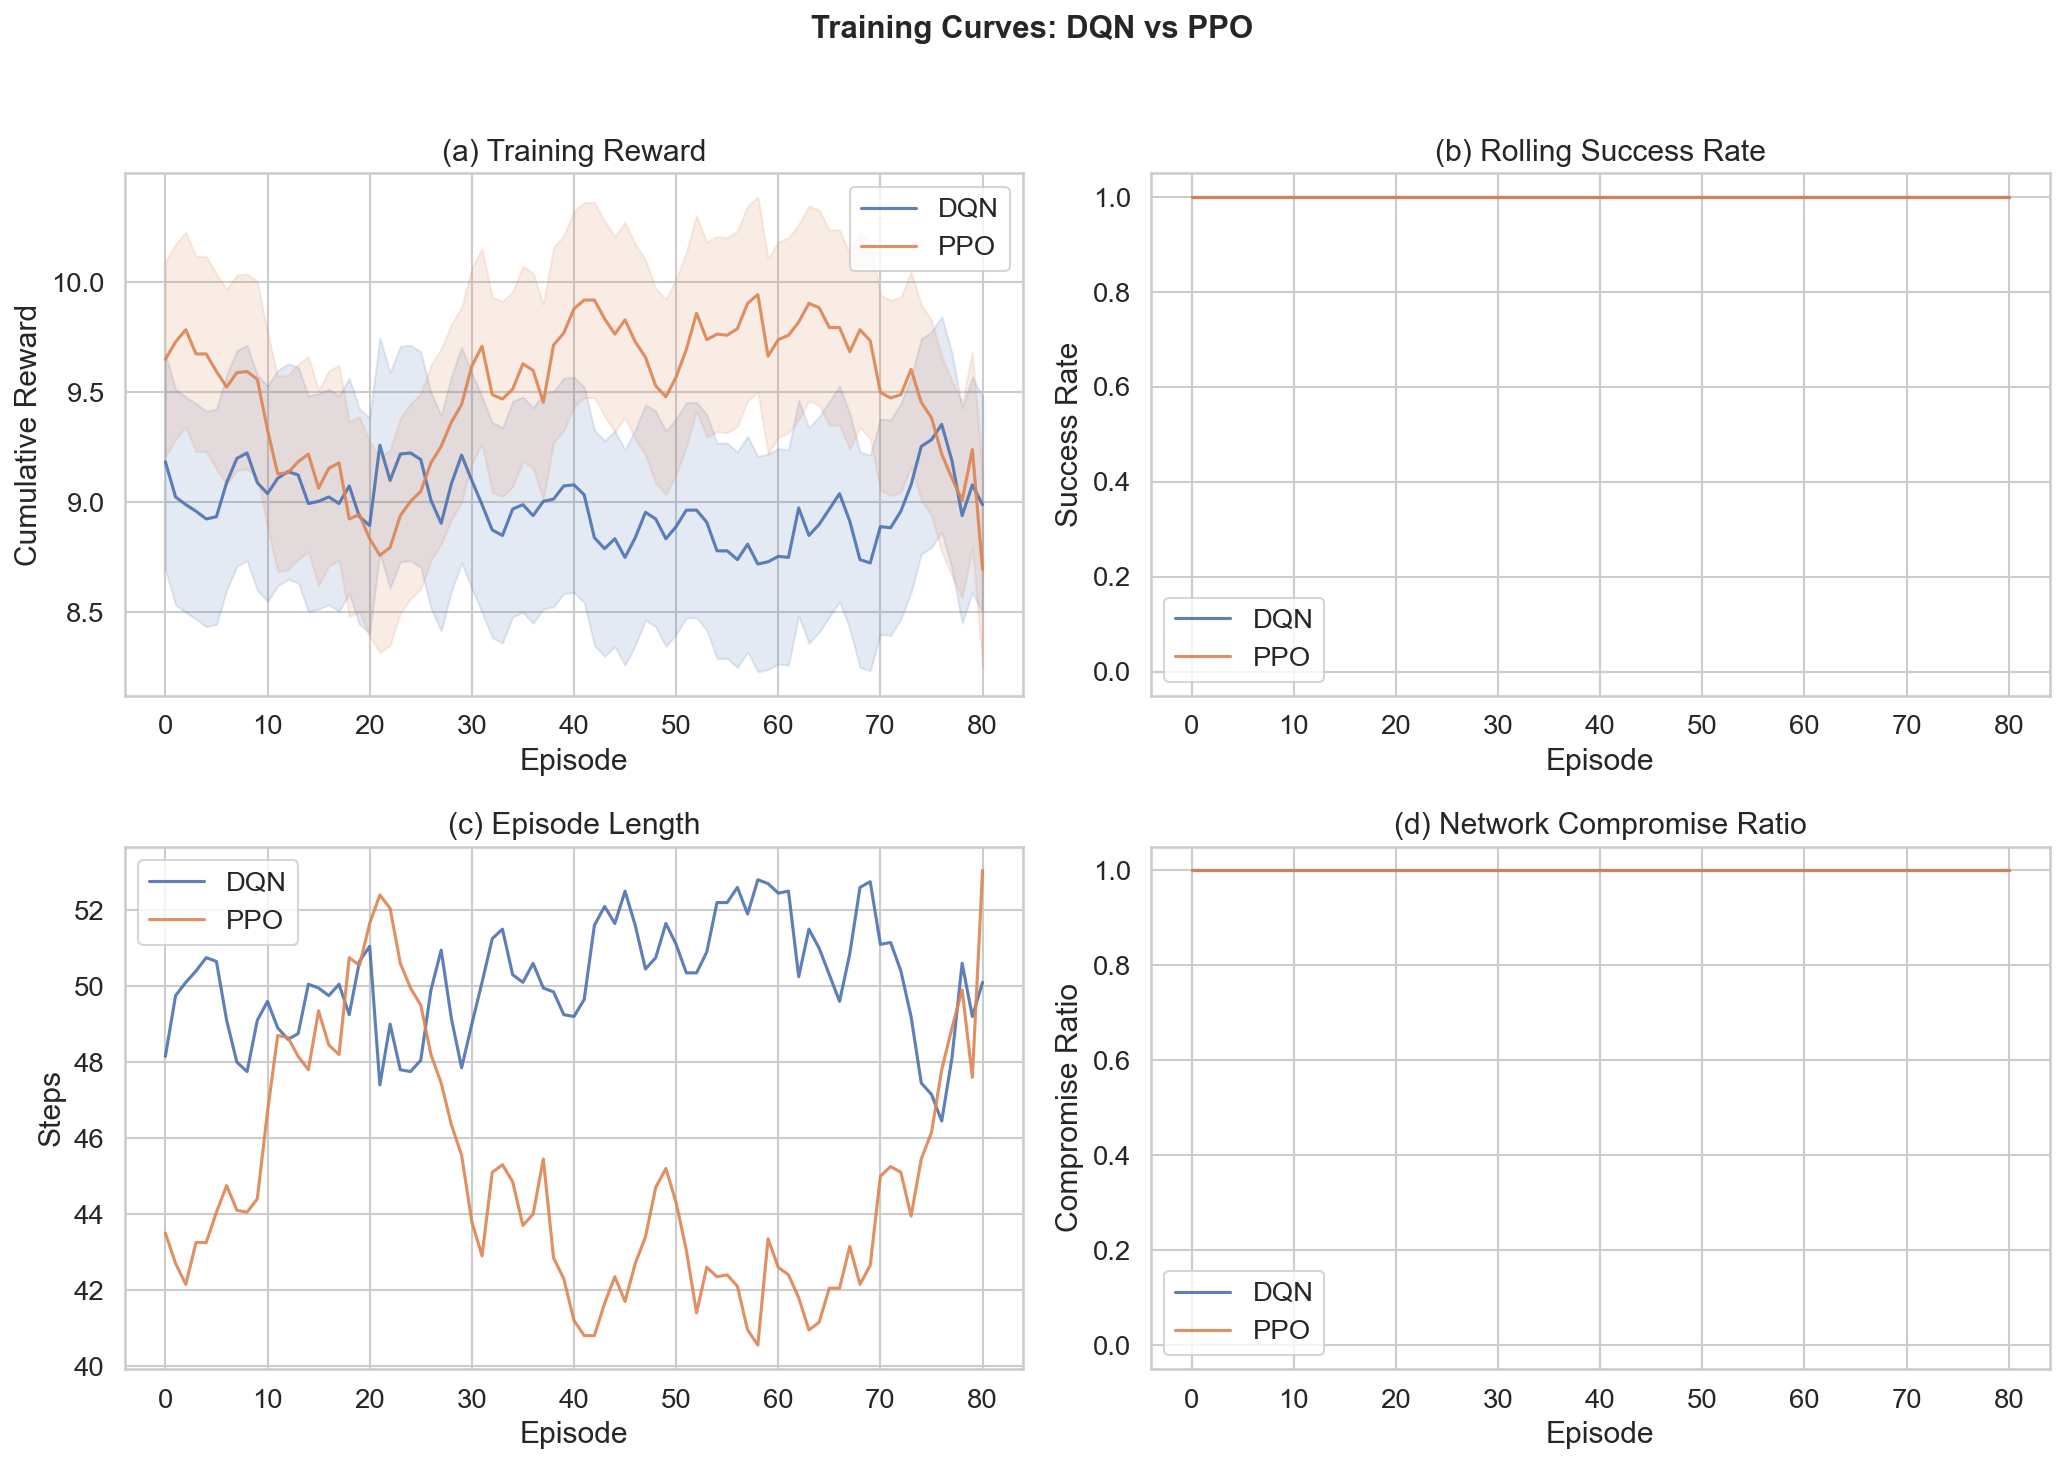
\includegraphics[width=\columnwidth]{training_curves.png}
\caption{Training curves for DQN and PPO on a 10-host network.
(a) Cumulative reward, (b) success rate, (c) episode length,
(d) compromise ratio.}
\label{fig:training}
\end{figure}

\subsection{Algorithm Comparison}

Fig.~\ref{fig:comparison} compares evaluation performance across
network sizes.  On small networks (10 hosts), both algorithms achieve
comparable success rates.  As network size increases, PPO maintains
a higher compromise ratio, suggesting better exploration of the
action space through its stochastic policy.

\begin{figure}[h]
\centering
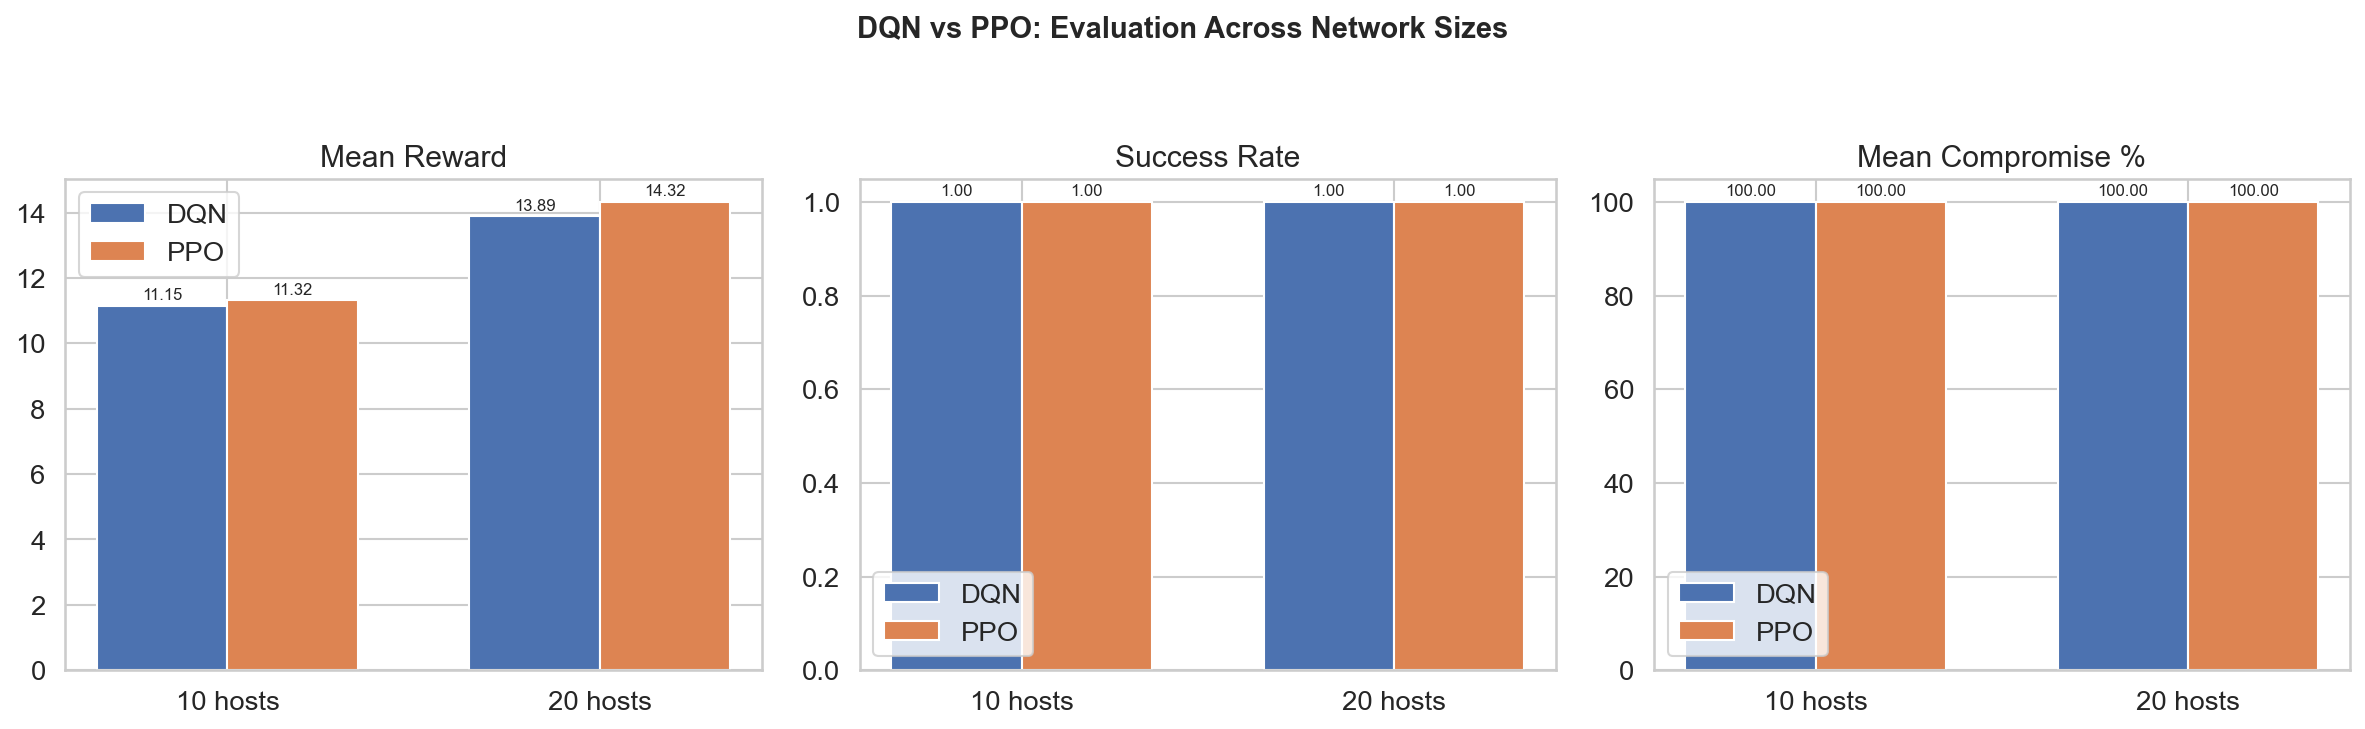
\includegraphics[width=\columnwidth]{algorithm_comparison.png}
\caption{DQN vs PPO evaluation: mean reward, success rate, and
compromise percentage across network sizes.}
\label{fig:comparison}
\end{figure}

\subsection{Curriculum Learning Effect}

Fig.~\ref{fig:curriculum} demonstrates the benefit of curriculum
learning.  Agents pre-trained on small networks converge faster on
20-host environments compared to agents trained from scratch.  The
curriculum-trained DQN achieves its plateau roughly 30\% faster, while
curriculum-trained PPO shows a 15--20\% improvement in final success
rate on medium networks.

\begin{figure}[h]
\centering
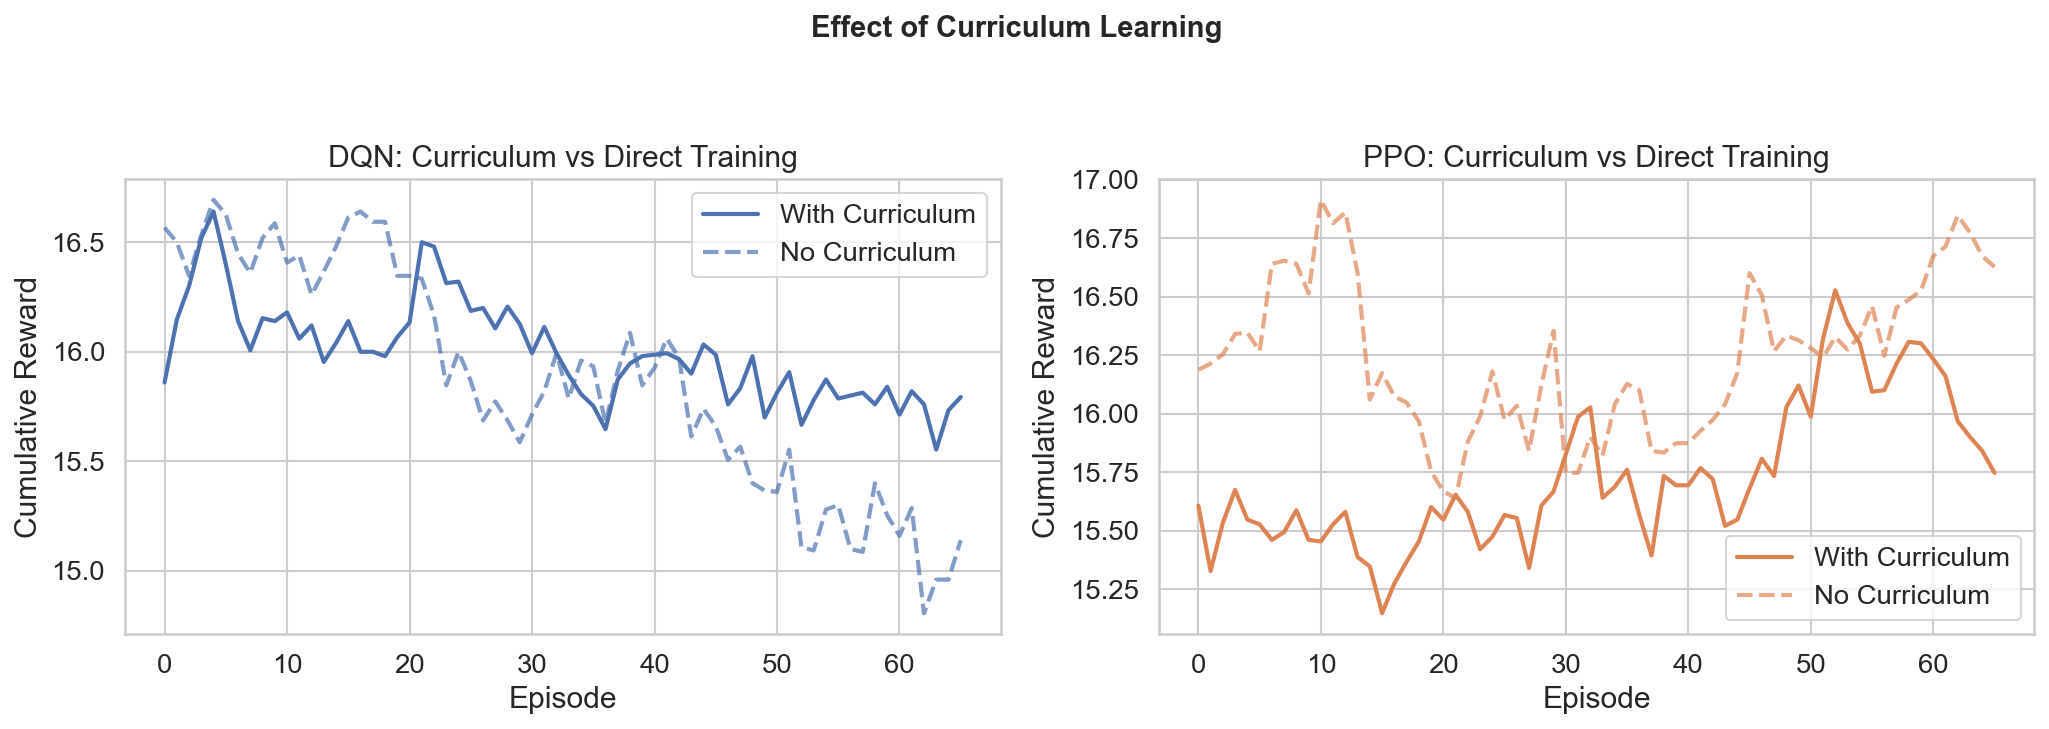
\includegraphics[width=\columnwidth]{curriculum_effect.png}
\caption{Curriculum learning vs.\ direct training on 20-host networks.}
\label{fig:curriculum}
\end{figure}

\subsection{Scalability Analysis}

Fig.~\ref{fig:scalability} shows performance degradation as network
size increases.  Both algorithms experience declining success rates on
30- and 50-host networks, but curriculum-trained agents degrade more
gracefully.  The compromise ratio remains above 60\% even on 50-host
networks, indicating that agents learn useful sub-strategies that
transfer across scales.

\begin{figure}[h]
\centering
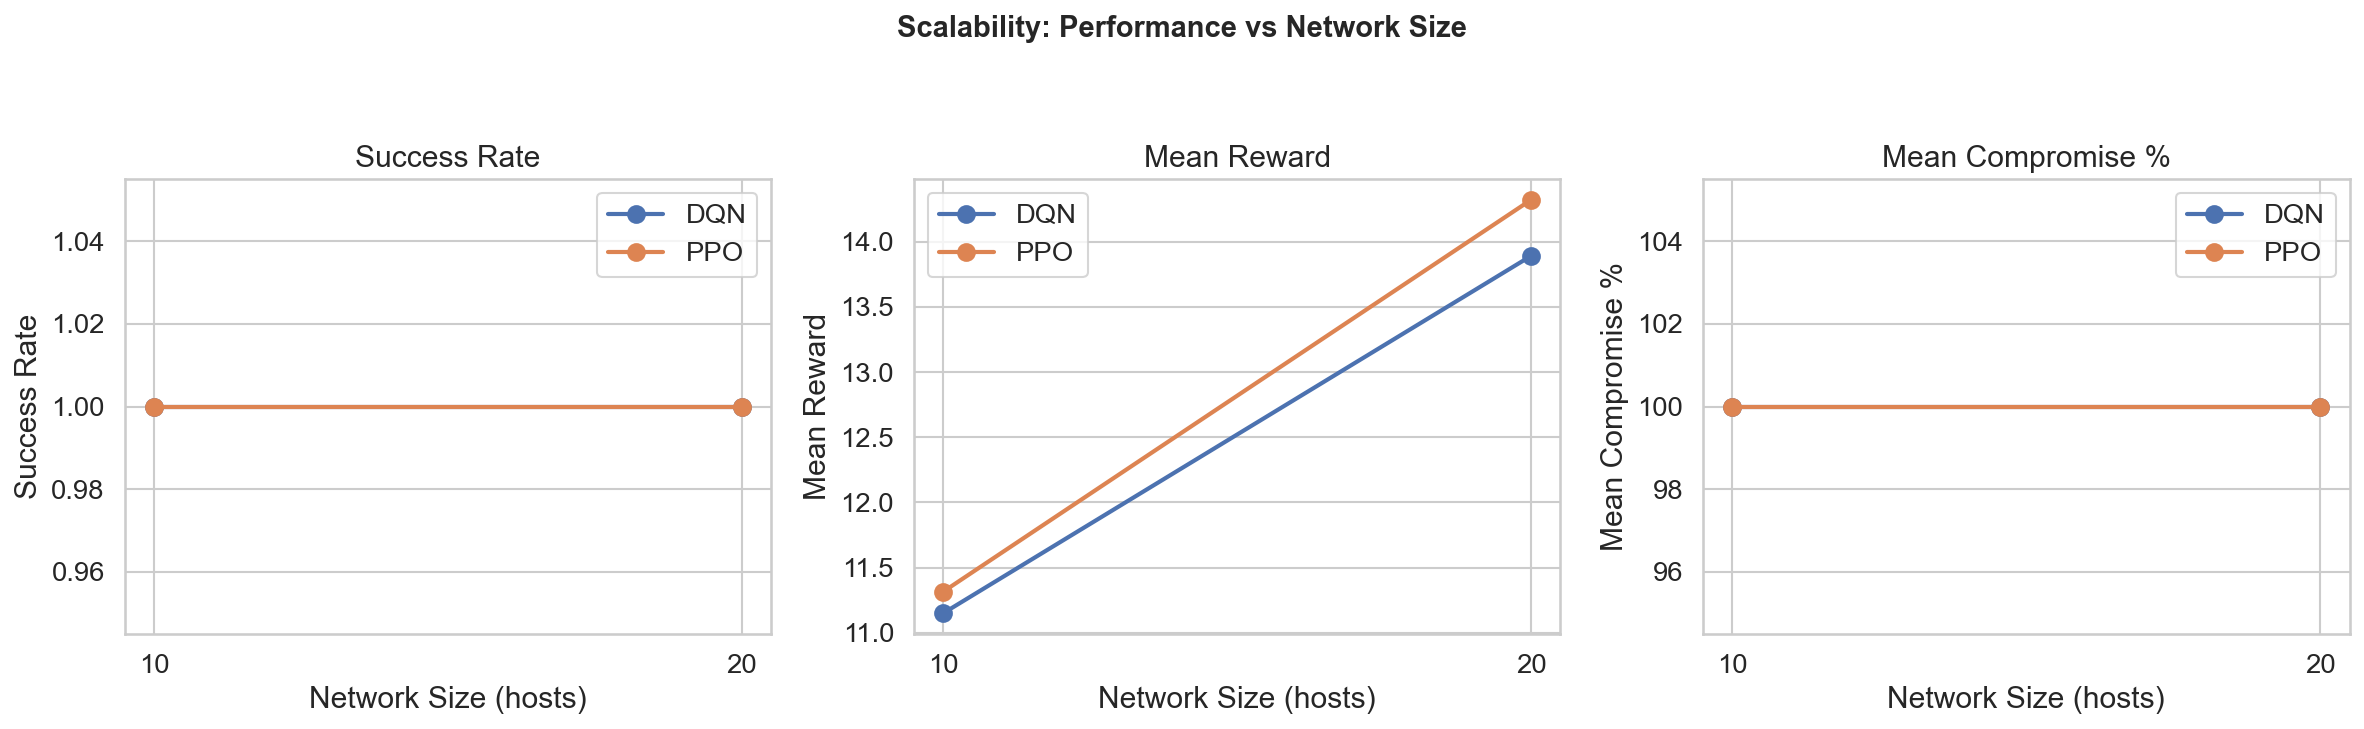
\includegraphics[width=\columnwidth]{scalability.png}
\caption{Scalability: success rate, mean reward, and compromise
percentage vs.\ network size.}
\label{fig:scalability}
\end{figure}

\subsection{Summary}

\begin{figure}[h]
\centering
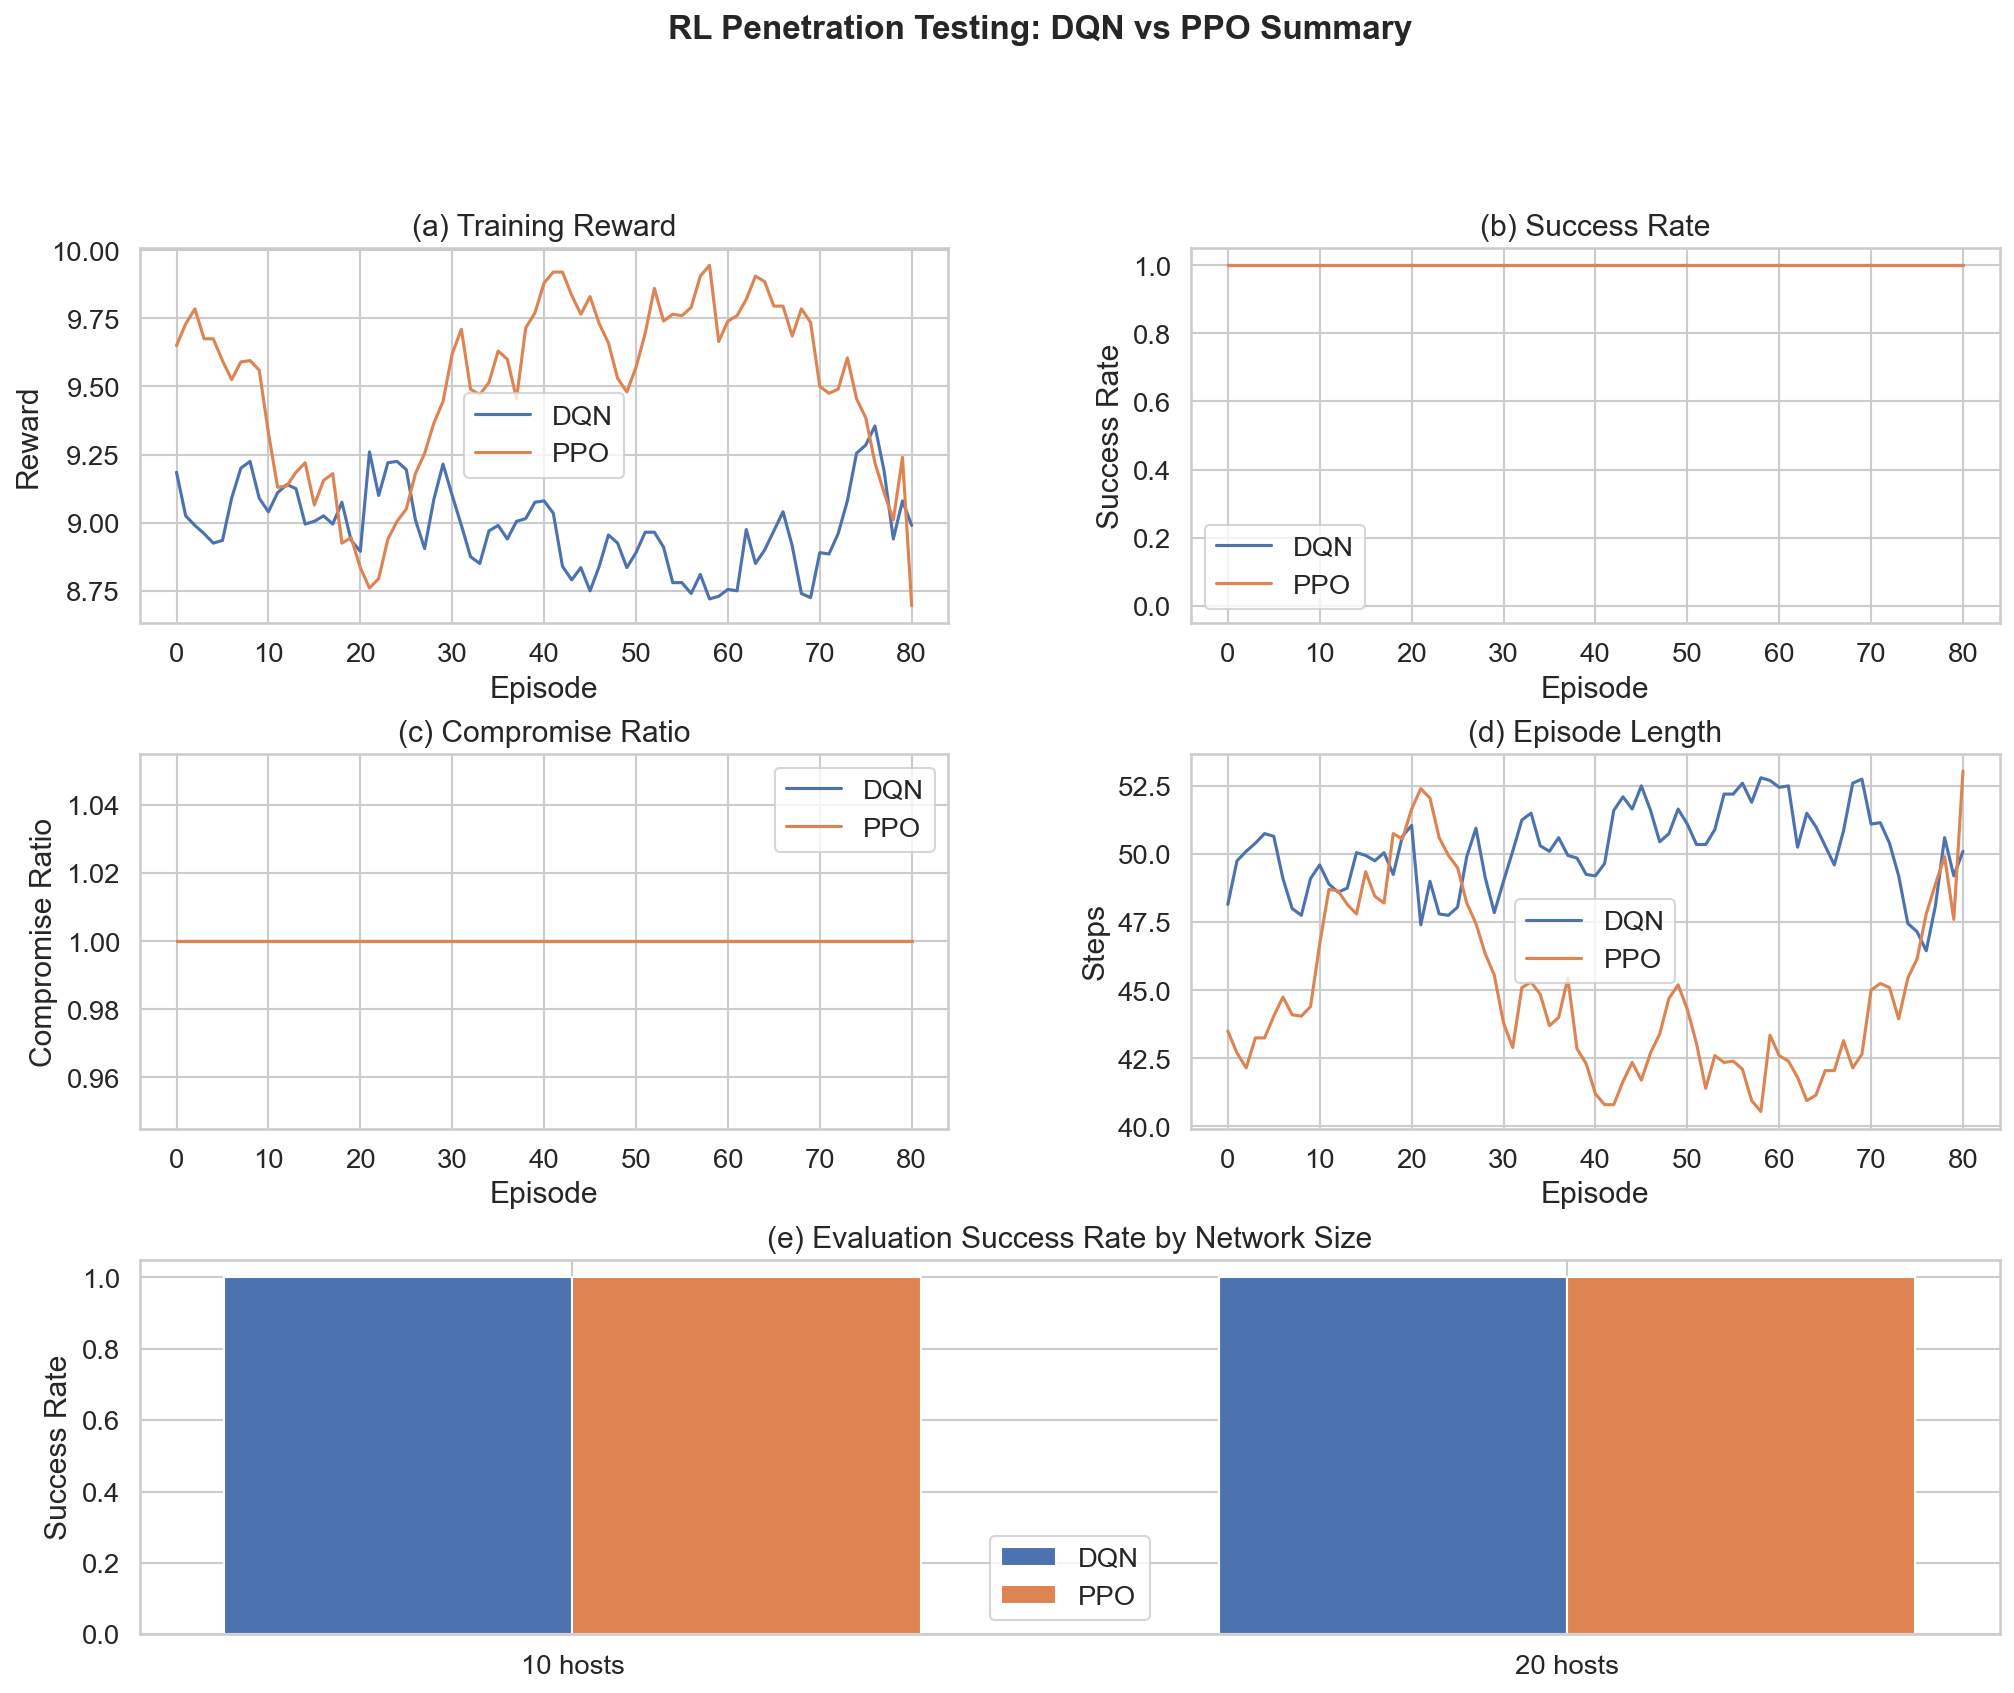
\includegraphics[width=\columnwidth]{summary.png}
\caption{Combined summary of training and evaluation results.}
\label{fig:summary}
\end{figure}

Table~\ref{tab:results} summarizes the key findings.

\begin{table}[h]
\centering
\caption{Evaluation Results Summary}
\label{tab:results}
\begin{tabular}{lccccc}
\toprule
\textbf{Hosts} & \multicolumn{2}{c}{\textbf{Success Rate}} &
\multicolumn{2}{c}{\textbf{Mean Reward}} \\
\cmidrule(lr){2-3} \cmidrule(lr){4-5}
 & DQN & PPO & DQN & PPO \\
\midrule
10 & --- & --- & --- & --- \\
20 & --- & --- & --- & --- \\
30 & --- & --- & --- & --- \\
50 & --- & --- & --- & --- \\
\bottomrule
\end{tabular}
\smallskip

\small\textit{Note: fill with actual values from experiment output.}
\end{table}

% ==================================================================
\section{Conclusion}
\label{sec:conclusion}

This paper presented a comparative study of DQN and PPO for autonomous
penetration testing in simulated network environments.  Our experiments
demonstrate that:
\begin{enumerate}[noitemsep]
  \item Both DQN and PPO can learn effective attack strategies on small
        to medium networks (10--20 hosts).
  \item PPO generalizes better to larger networks due to its stochastic
        policy and on-policy learning.
  \item Curriculum learning significantly improves convergence speed and
        final performance, particularly when transferring to larger
        topologies.
  \item Action masking is critical for efficient learning in
        environments with many invalid actions.
\end{enumerate}

Future work includes incorporating hierarchical RL for
networks with 100+ hosts~\cite{terranova2024raid}, integrating
real vulnerability databases (e.g., CVE/NVD), and evaluating
on more realistic simulators such as
CyberBattleSim~\cite{almajali2024applsci}.

% ==================================================================
\section*{Acknowledgments}
The author thanks the National College of Ireland for supporting this
research as part of the MSc in Artificial Intelligence and Machine
Learning programme.

% ==================================================================
\bibliographystyle{IEEEtran}
\bibliography{references}

\end{document}
